
\section{Resultados}

El término HPO HP:0012347, \textit{Abnormal protein N-linked glycosylation} (alteración de la N-glicosilación de proteínas), está asociado a 50 genes. Los 50 genes se mapearon en STRING \cite{Szklarczyk2023} (versión 12.5, taxón 9606). Con un umbral de puntuación de 800, 41 genes formaron una red con 106 aristas; los 9 genes restantes no tuvieron interacciones que superaran ese umbral. La red presentó una transitividad global de 0.6263 y quedó dividida en 3 componentes conexas.

\subsection{Clustering de la red}
Aplicamos el algoritmo de Louvain \cite{Blondel2008} (semilla 123) a la red de 41 nodos, que la dividió en 7 clusters (Figura~\ref{fig:clusters} y Tabla~\ref{tab:clusters}). Cuatro de ellos tienen al menos 5 genes. El cluster 1 (11 genes) reúne a \textit{ALG1}, \textit{ALG2}, \textit{ALG3}, \textit{ALG6}, \textit{ALG8}, \textit{ALG9}, \textit{ALG11}, \textit{ALG12}, \textit{ALG13}, \textit{PMM2} y \textit{RFT1}. El cluster 2 (8 genes) contiene \textit{DPAGT1}, \textit{DHRSX}, \textit{DOLK}, \textit{DPM1}, \textit{DPM2}, \textit{DPM3}, \textit{MPDU1} y \textit{SRD5A3}. El cluster 3 (6 genes) está formado por \textit{ATP6AP1}, \textit{ATP6AP2}, \textit{ATP6V0A2}, \textit{ATP6V1A}, \textit{ATP6V1E1} y \textit{VMA12}, y el cluster 4 (7 genes) por \textit{COG1} y \textit{COG3} a \textit{COG8}. Los tres clusters restantes son pequeños: \textit{GET4} y \textit{CAMLG} (2 genes), \textit{MPI}, \textit{PGM1} y \textit{PGM2L1} (3 genes), y \textit{DDOST}, \textit{EDEM3}, \textit{MAGT1} y \textit{SSR4} (4 genes).

\begin{figure}[htbp]
	\centering
	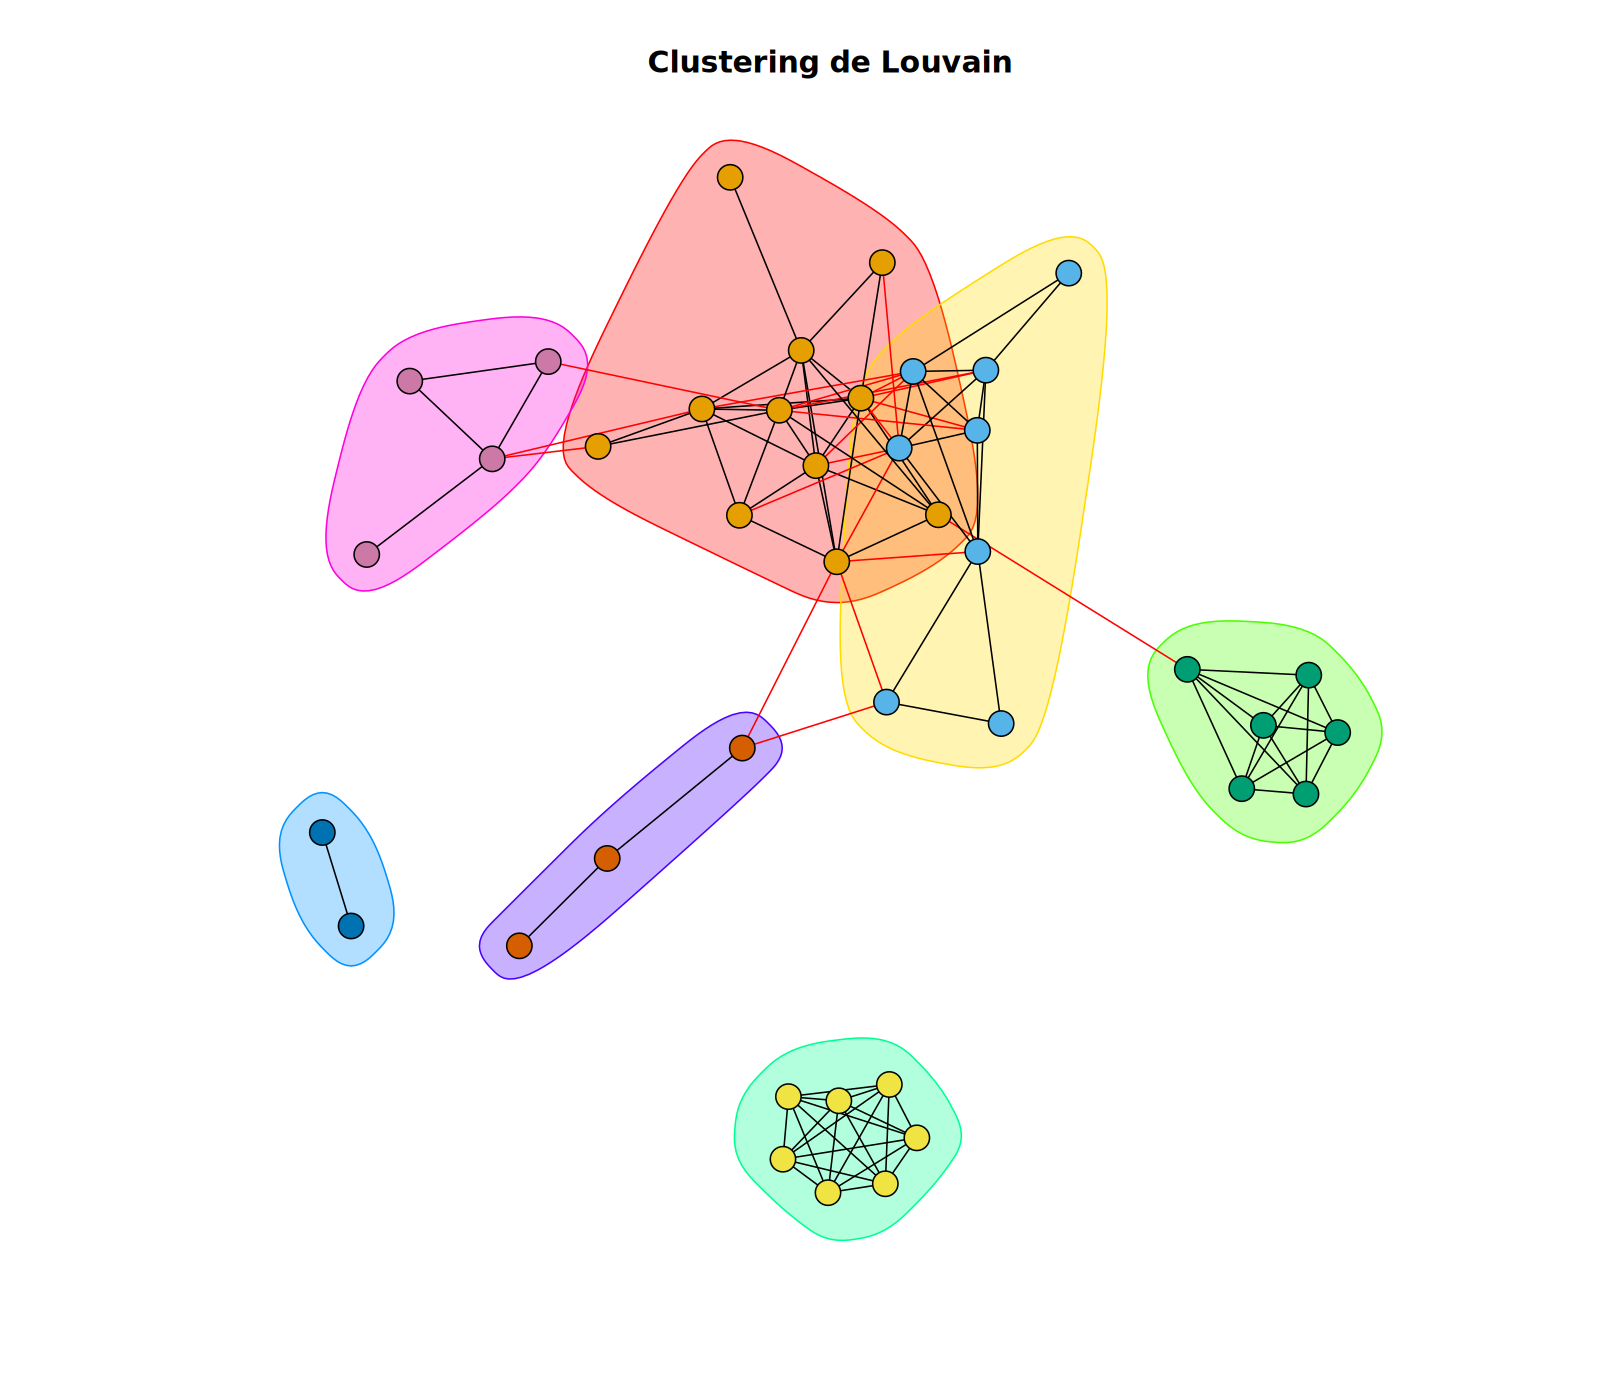
\includegraphics[width=0.9\textwidth]{figures/red_clusters.png}
	\caption{Red de interacciones de STRING (puntuación $\geq$ 800) entre los genes asociados al HP:0012347, coloreada según los clusters de Louvain.}
	\label{fig:clusters}
\end{figure}

\subsection{Enriquecimiento funcional}
Realizamos un análisis de sobrerrepresentación (ORA) de términos de Gene Ontology (procesos biológicos) con \textit{clusterProfiler} \cite{Yu2012}, usando la corrección de Benjamini-Hochberg \cite{BenjaminiHochberg1995} y un umbral de p-valor ajustado de 0,05. Para los 50 genes del HPO, con todos los genes humanos anotados como fondo, obtuvimos 79 términos enriquecidos. Los más significativos fueron \textit{protein N-linked glycosylation} (22 de 50 genes; p ajustado $3{,}2\times10^{-37}$), \textit{glycoprotein metabolic process} (27/50; $3{,}6\times10^{-31}$), \textit{dolichol-linked oligosaccharide biosynthetic process} (14/50; $4{,}6\times10^{-31}$) y \textit{glycoprotein biosynthetic process} (25/50; $5{,}1\times10^{-30}$). También apareció \textit{intra-Golgi vesicle-mediated transport} (7/50; $2{,}4\times10^{-10}$).

Para cada cluster de al menos 5 genes repetimos el análisis tomando como fondo los 41 genes de la red (Tabla~\ref{tab:clusters}). El cluster 1 se enriqueció en \textit{protein N-linked glycosylation} (11/11) y en \textit{dolichol-linked oligosaccharide biosynthetic process} (10/11). El cluster 4 se enriqueció en términos de transporte y localización de proteínas, como \textit{intracellular protein localization} y \textit{vesicle-mediated transport} (7/7). El cluster 2 solo mostró términos genéricos de metabolismo de fosfato (6/8), y el cluster 3 un único término muy general, \textit{biological regulation} (6/6).

\begin{table}[htbp]
	\caption{Clusters de Louvain con al menos 5 genes y término GO más significativo de cada uno.}
	\label{tab:clusters}
	\begin{tabular}{rrp{6cm}r}
		\hline
		Cluster & Genes & Término GO principal & p ajustado \\
		\hline
		1 & 11 & protein N-linked glycosylation & $9{,}8\times10^{-5}$ \\
		2 & 8 & phosphorus metabolic process & $7{,}1\times10^{-3}$ \\
		3 & 6 & biological regulation & $2{,}9\times10^{-2}$ \\
		4 & 7 & intracellular protein localization & $1{,}8\times10^{-4}$ \\
		\hline
	\end{tabular}
\end{table}

\subsection{Caracterización topológica y
dispersión de la red}

La red de asociaciones proteicas correspondiente
al fenotipo HP:0012347, construida mediante
STRING v12.5 con un umbral de confianza de 800,
estuvo formada por 41 nodos y 106 aristas,
distribuidos en tres componentes conexas.

La densidad de la red fue de 0.1293 y la
transitividad global de 0.6263.

El grado medio de los nodos fue de 5.1707,
con una mediana de 5 y una desviación típica
de 2.7559. La varianza del grado fue de
7.5951 y el coeficiente de variación alcanzó
el 53.30\%.

El grado mínimo fue de 1 y el máximo de 11.
El primer y tercer cuartil fueron 3 y 6,
respectivamente.

Estos resultados muestran una distribución
heterogénea del número de asociaciones
entre las proteínas analizadas.

\begin{table}[htbp]
\centering
\caption{Medidas topológicas y de dispersión
de la red HP:0012347.}
\label{tab:dispersion_red}

\begin{tabular}{lc}
\hline
Medida & Valor \\
\hline
Nodos & 41 \\
Aristas & 106 \\
Componentes conexas & 3 \\
Densidad & 0.1293 \\
Transitividad & 0.6263 \\
Grado medio & 5.1707 \\
Mediana & 5 \\
Varianza & 7.5951 \\
Desviación típica & 2.7559 \\
Coeficiente de variación & 53.30\% \\
Grado mínimo & 1 \\
Grado máximo & 11 \\
Primer cuartil & 3 \\
Tercer cuartil & 6 \\
\hline
\end{tabular}
\end{table}

\begin{figure}[htbp]
\centering
\includegraphics[width=0.85\textwidth]
{../results/analisis_avanzado/distribucion_grado.pdf}
\caption{Distribución del grado de los nodos de
la red HP:0012347. La línea discontinua
representa el grado medio.}
\label{fig:distribucion_grado}
\end{figure}

\begin{figure}[htbp]
\centering
\includegraphics[width=0.75\textwidth]
{../results/analisis_avanzado/boxplot_grado.pdf}
\caption{Diagrama de cajas de la distribución
del grado de los nodos de la red.}
\label{fig:boxplot_grado}
\end{figure}

\subsubsection{Identificación de proteínas con mayor conectividad}

El análisis del grado permitió identificar las proteínas
con mayor número de asociaciones directas dentro de la
red. Como se observa en la Figura~\ref{fig:top10_grado},
los genes \textit{ALG1} y \textit{ALG3} presentaron el
mayor grado, con 11 conexiones cada uno.

Los genes \textit{ALG6}, \textit{PMM2}, \textit{DPM1}
y \textit{DPAGT1} presentaron 9 conexiones, seguidos
de \textit{ALG12} y \textit{ALG11}, con 8 conexiones,
y \textit{DPM2} y \textit{DOLK}, con 7 conexiones.

Los genes ALG1 y ALG3 presentaron una conectividad
superior al doble del grado medio de la red, lo que
permite identificarlos como candidatos a hubs.

\begin{figure}[htbp]
    \centering
    \includegraphics[width=0.85\textwidth]
    {../results/analisis_avanzado/top10_grado.pdf}
    \caption{Diez proteínas con mayor grado en la red
    de asociaciones proteicas del fenotipo HP:0012347.}
    \label{fig:top10_grado}
\end{figure}



\subsection{Análisis de centralidades y proteínas puente}

El análisis de centralidades permitió identificar
proteínas relevantes según diferentes criterios
estructurales, más allá del número de asociaciones
directas.

Los genes \textit{ALG1} y \textit{ALG3} destacaron
en varias medidas de centralidad. ALG1 presentó los
mayores valores de centralidad armónica (0.4813),
cercanía (0.5000) y autovector (1.0000), mientras
que ALG3 obtuvo el mayor valor de PageRank (0.0447).

Sin embargo, el mayor valor de intermediación
correspondió a \textit{ALG2} (0.1960), seguido
de \textit{ATP6V0A2} (0.1667) y \textit{PMM2}
(0.1518).

\begin{table}[htbp]
\centering
\caption{Genes con mayor puntuación en cada medida
de centralidad y conectividad entre comunidades.}
\label{tab:centralidades_maximas}
\begin{tabular}{lcr}
\hline
Medida & Gen & Valor \\
\hline
Grado & ALG1, ALG3 & 11 \\
Intermediación & ALG2 & 0.1960 \\
Armónica & ALG1 & 0.4813 \\
Cercanía & ALG1 & 0.5000 \\
Autovector & ALG1 & 1.0000 \\
PageRank & ALG3 & 0.0447 \\
Participación & MPI & 0.6667 \\
Conexiones externas & DPAGT1 & 5 \\
\hline
\end{tabular}
\end{table}

\subsubsection{Conectividad entre comunidades}

El mayor coeficiente de participación correspondió
al gen \textit{MPI} (0.6667), seguido de
\textit{SRD5A3} (0.6250) y \textit{PMM2} (0.5679).

Por otro lado, \textit{DPAGT1} presentó el mayor
número de conexiones externas, con cinco asociaciones
con proteínas pertenecientes a otras comunidades.

La modularidad de la partición de Louvain fue de
0.5688.

Se identificaron seis puntos de articulación:
\textit{ALG11}, \textit{ATP6V0A2}, \textit{ALG2},
\textit{DDOST}, \textit{PGM2L1} y \textit{MPI}.

La eliminación individual de cualquiera de estos
nodos incrementa el número de componentes conexas
de la red.

\begin{figure}[htbp]
    \centering
    \includegraphics[width=0.95\textwidth]
    {../results/analisis_avanzado/red_intermediacion.pdf}
    \caption{Red coloreada según las comunidades
    de Louvain. El tamaño de los nodos es proporcional
    a su centralidad de intermediación. Los bordes
    rojos identifican los puntos de articulación.}
    \label{fig:red_intermediacion}
\end{figure}

\subsubsection{Relación entre las medidas de centralidad}

El análisis de correlación de Spearman mostró una
elevada concordancia entre el grado y PageRank
($\rho=0.906$), así como entre el coeficiente de
participación y las conexiones externas
($\rho=0.964$).

Por el contrario, la correlación entre grado e
intermediación fue moderada ($\rho=0.523$), mientras
que la correlación entre grado y participación
fue de 0.410.

Estos resultados muestran que las medidas analizadas
proporcionan información parcialmente complementaria
sobre la organización estructural de la red.

\begin{figure}[htbp]
    \centering
    \includegraphics[width=0.9\textwidth]
    {../results/analisis_avanzado/correlaciones_centralidad.pdf}
    \caption{Matriz de correlaciones de Spearman
    entre las medidas de centralidad y conectividad
    entre comunidades.}
    \label{fig:correlaciones_centralidad}
\end{figure}

\begin{figure}[htbp]
    \centering
    \includegraphics[width=0.85\textwidth]
    {../results/analisis_avanzado/grado_intermediacion.pdf}
    \caption{Relación entre el grado y la centralidad
    de intermediación de los nodos. Los colores
    representan las comunidades de Louvain.}
    \label{fig:grado_intermediacion}
\end{figure}
